% Options for packages loaded elsewhere
\PassOptionsToPackage{unicode}{hyperref}
\PassOptionsToPackage{hyphens}{url}
%
\documentclass[
]{article}
\usepackage{amsmath,amssymb}
\usepackage{lmodern}
\usepackage{ifxetex,ifluatex}
\ifnum 0\ifxetex 1\fi\ifluatex 1\fi=0 % if pdftex
  \usepackage[T1]{fontenc}
  \usepackage[utf8]{inputenc}
  \usepackage{textcomp} % provide euro and other symbols
\else % if luatex or xetex
  \usepackage{unicode-math}
  \defaultfontfeatures{Scale=MatchLowercase}
  \defaultfontfeatures[\rmfamily]{Ligatures=TeX,Scale=1}
\fi
% Use upquote if available, for straight quotes in verbatim environments
\IfFileExists{upquote.sty}{\usepackage{upquote}}{}
\IfFileExists{microtype.sty}{% use microtype if available
  \usepackage[]{microtype}
  \UseMicrotypeSet[protrusion]{basicmath} % disable protrusion for tt fonts
}{}
\makeatletter
\@ifundefined{KOMAClassName}{% if non-KOMA class
  \IfFileExists{parskip.sty}{%
    \usepackage{parskip}
  }{% else
    \setlength{\parindent}{0pt}
    \setlength{\parskip}{6pt plus 2pt minus 1pt}}
}{% if KOMA class
  \KOMAoptions{parskip=half}}
\makeatother
\usepackage{xcolor}
\IfFileExists{xurl.sty}{\usepackage{xurl}}{} % add URL line breaks if available
\IfFileExists{bookmark.sty}{\usepackage{bookmark}}{\usepackage{hyperref}}
\hypersetup{
  pdftitle={Economics Club Introduction to R Example},
  pdfauthor={Jason Smith - GVSU Economics Club},
  hidelinks,
  pdfcreator={LaTeX via pandoc}}
\urlstyle{same} % disable monospaced font for URLs
\usepackage[margin=1in]{geometry}
\usepackage{color}
\usepackage{fancyvrb}
\newcommand{\VerbBar}{|}
\newcommand{\VERB}{\Verb[commandchars=\\\{\}]}
\DefineVerbatimEnvironment{Highlighting}{Verbatim}{commandchars=\\\{\}}
% Add ',fontsize=\small' for more characters per line
\usepackage{framed}
\definecolor{shadecolor}{RGB}{248,248,248}
\newenvironment{Shaded}{\begin{snugshade}}{\end{snugshade}}
\newcommand{\AlertTok}[1]{\textcolor[rgb]{0.94,0.16,0.16}{#1}}
\newcommand{\AnnotationTok}[1]{\textcolor[rgb]{0.56,0.35,0.01}{\textbf{\textit{#1}}}}
\newcommand{\AttributeTok}[1]{\textcolor[rgb]{0.77,0.63,0.00}{#1}}
\newcommand{\BaseNTok}[1]{\textcolor[rgb]{0.00,0.00,0.81}{#1}}
\newcommand{\BuiltInTok}[1]{#1}
\newcommand{\CharTok}[1]{\textcolor[rgb]{0.31,0.60,0.02}{#1}}
\newcommand{\CommentTok}[1]{\textcolor[rgb]{0.56,0.35,0.01}{\textit{#1}}}
\newcommand{\CommentVarTok}[1]{\textcolor[rgb]{0.56,0.35,0.01}{\textbf{\textit{#1}}}}
\newcommand{\ConstantTok}[1]{\textcolor[rgb]{0.00,0.00,0.00}{#1}}
\newcommand{\ControlFlowTok}[1]{\textcolor[rgb]{0.13,0.29,0.53}{\textbf{#1}}}
\newcommand{\DataTypeTok}[1]{\textcolor[rgb]{0.13,0.29,0.53}{#1}}
\newcommand{\DecValTok}[1]{\textcolor[rgb]{0.00,0.00,0.81}{#1}}
\newcommand{\DocumentationTok}[1]{\textcolor[rgb]{0.56,0.35,0.01}{\textbf{\textit{#1}}}}
\newcommand{\ErrorTok}[1]{\textcolor[rgb]{0.64,0.00,0.00}{\textbf{#1}}}
\newcommand{\ExtensionTok}[1]{#1}
\newcommand{\FloatTok}[1]{\textcolor[rgb]{0.00,0.00,0.81}{#1}}
\newcommand{\FunctionTok}[1]{\textcolor[rgb]{0.00,0.00,0.00}{#1}}
\newcommand{\ImportTok}[1]{#1}
\newcommand{\InformationTok}[1]{\textcolor[rgb]{0.56,0.35,0.01}{\textbf{\textit{#1}}}}
\newcommand{\KeywordTok}[1]{\textcolor[rgb]{0.13,0.29,0.53}{\textbf{#1}}}
\newcommand{\NormalTok}[1]{#1}
\newcommand{\OperatorTok}[1]{\textcolor[rgb]{0.81,0.36,0.00}{\textbf{#1}}}
\newcommand{\OtherTok}[1]{\textcolor[rgb]{0.56,0.35,0.01}{#1}}
\newcommand{\PreprocessorTok}[1]{\textcolor[rgb]{0.56,0.35,0.01}{\textit{#1}}}
\newcommand{\RegionMarkerTok}[1]{#1}
\newcommand{\SpecialCharTok}[1]{\textcolor[rgb]{0.00,0.00,0.00}{#1}}
\newcommand{\SpecialStringTok}[1]{\textcolor[rgb]{0.31,0.60,0.02}{#1}}
\newcommand{\StringTok}[1]{\textcolor[rgb]{0.31,0.60,0.02}{#1}}
\newcommand{\VariableTok}[1]{\textcolor[rgb]{0.00,0.00,0.00}{#1}}
\newcommand{\VerbatimStringTok}[1]{\textcolor[rgb]{0.31,0.60,0.02}{#1}}
\newcommand{\WarningTok}[1]{\textcolor[rgb]{0.56,0.35,0.01}{\textbf{\textit{#1}}}}
\usepackage{graphicx}
\makeatletter
\def\maxwidth{\ifdim\Gin@nat@width>\linewidth\linewidth\else\Gin@nat@width\fi}
\def\maxheight{\ifdim\Gin@nat@height>\textheight\textheight\else\Gin@nat@height\fi}
\makeatother
% Scale images if necessary, so that they will not overflow the page
% margins by default, and it is still possible to overwrite the defaults
% using explicit options in \includegraphics[width, height, ...]{}
\setkeys{Gin}{width=\maxwidth,height=\maxheight,keepaspectratio}
% Set default figure placement to htbp
\makeatletter
\def\fps@figure{htbp}
\makeatother
\setlength{\emergencystretch}{3em} % prevent overfull lines
\providecommand{\tightlist}{%
  \setlength{\itemsep}{0pt}\setlength{\parskip}{0pt}}
\setcounter{secnumdepth}{-\maxdimen} % remove section numbering
\usepackage{float} \floatplacement{figure}{H} \floatplacement{table}{H}
\usepackage{booktabs}
\usepackage{longtable}
\usepackage{array}
\usepackage{multirow}
\usepackage{wrapfig}
\usepackage{float}
\usepackage{colortbl}
\usepackage{pdflscape}
\usepackage{tabu}
\usepackage{threeparttable}
\usepackage{threeparttablex}
\usepackage[normalem]{ulem}
\usepackage{makecell}
\usepackage{xcolor}
\ifluatex
  \usepackage{selnolig}  % disable illegal ligatures
\fi

\title{Economics Club Introduction to R Example}
\author{Jason Smith - GVSU Economics Club}
\date{}

\begin{document}
\maketitle

\hypertarget{introduction}{%
\subsection{Introduction}\label{introduction}}

This is the companion document for the Introduction to R code that was
presented at the Economics Club meeting. My intention for this is to be
some form of ``director's cut'' where I can explain a bit in a bit more
detail what's going on. Some alterations have been made to the code to
better show things in document form. I think the best way to learn R is
by using R. I hope this document is helpful jumping off point.

\hypertarget{getting-help}{%
\subsection{Getting Help}\label{getting-help}}

R is unlike any software package most people have used in the past.
While R give us the freedom to perform more complex analysis than
programs like Excel, it's also easier for new users to make mistakes.
When your code won't run, try not to get frustrated. Every error is an
opportunity to learn something new about R and will ultimately make you
a better programmer. You can't get better if you don't make mistakes!\\
When you get an error, read the error message carefully. They can often
help you determine what the problem is. You can also copy/paste the
message into Google and find help online. You're probably not the first
person to run into that error!\\
This may not sound like useful advice, but it's so important to at the
very least skim through the documentation for a function if you don't
know how to use it. In R you can do this in the console by typing
\texttt{?FUNCTION\_NAME} and pressing enter. This will pull up the
documentation in the bottom right. The documentation will tell you what
arguments the function accepts and how they work. There are often
examples at the very bottom of the page. You can also find documentation
at \url{www.rdocumentation.org}.\\
The internet also has a lot of resources for learning R. Googling what
you're trying to do in R or the package you're working with will often
provide instructions and code examples. Not all of it will be relevant
for what you're doing in the moment so it's important to read for a
variety of sources and experiment to find what works.

\hypertarget{data-background}{%
\subsection{Data Background}\label{data-background}}

The data used in this document comes from the \emph{palmer penguin}
package available \url{www.github.com/allisonhorst/palmerpenguins}. It
contains body measurements for 344 penguins. The codebook follows

\begin{table}

\caption{\label{tab:unnamed-chunk-1}Codebook}
\centering
\begin{tabular}[t]{ll}
\toprule
Variable & Meaning\\
\midrule
\cellcolor{gray!6}{Species} & \cellcolor{gray!6}{The species of the penguin (Adelie, Chinstrap, Gentoo)}\\
island & Island where penguin lives (Biscoe, Dream, Torgenson)\\
\cellcolor{gray!6}{bill.length.mm} & \cellcolor{gray!6}{Length of the bill in millimeters}\\
bill.depth.mm & Depth (or height) of the bill in millimeters\\
\cellcolor{gray!6}{body.mass.g} & \cellcolor{gray!6}{Body mass of the penguin in grams}\\
\addlinespace
sex & Sex of the penguin (male, female)\\
\cellcolor{gray!6}{year} & \cellcolor{gray!6}{Year the measurement was taken (2007, 2008, 2009)}\\
\bottomrule
\end{tabular}
\end{table}

\hypertarget{loading-packages}{%
\subsection{Loading Packages}\label{loading-packages}}

Packages are bits of shareable code. Typically, they'll contain datasets
or new functions so you don't have to program them yourself. The most
common way to install a package is with the command
\texttt{install.packages("PACKAGE\_NAME")}. You can then load the
package to be used in your code with the command
\texttt{library(PACKAGE\_NAME)}. In the majority of cases, you want to
start your code by loading all the packages you'll be using. By doing
this, you ensure your packages are properly loaded before you have to
use them. It also makes it easy for a collaborator to see what packages
you're using.

This code uses the following packages.

\begin{itemize}
  \item tidyverse: a collection of packages designed for data science
  \item texreg: summarizes regression output in publication ready tables
  \item vtable: easily creates publication ready tables
  \item ggpubr: wrapper for the *ggplot2* packages (included in the tidyverse) for publication ready graphics
\end{itemize}

\begin{Shaded}
\begin{Highlighting}[]
\FunctionTok{library}\NormalTok{(tidyverse)}
\FunctionTok{library}\NormalTok{(texreg)}
\FunctionTok{library}\NormalTok{(vtable)}
\FunctionTok{library}\NormalTok{(ggpubr)}
\end{Highlighting}
\end{Shaded}

\hypertarget{reading-in-data}{%
\subsection{Reading in Data}\label{reading-in-data}}

R can read data in a variety of formats. The easiest way to load your
data is using the \emph{import data} button in the environment tab. The
wizard will walk you through browsing for the file and importing it into
the environment. You can then copy and paste the import code into the
script file.

\begin{Shaded}
\begin{Highlighting}[]
\NormalTok{penguin }\OtherTok{\textless{}{-}} \FunctionTok{read\_csv}\NormalTok{(}\StringTok{"data/penguin.csv"}\NormalTok{)}
\end{Highlighting}
\end{Shaded}

\hypertarget{data-summaries}{%
\subsection{Data Summaries}\label{data-summaries}}

When you get a new dataset, a good way to begin to understand it is with
summary statistics. Before we start with that, we probably first want to
know how intact the data is. That is, do we have missing data? In this
dataset, we can click on the \emph{penguin} entry in the environment tab
to open it in a new window. In this case, we can quickly see some values
are missing (noted in R by \emph{NA}). To show this in document form,
below is some code that will create a table with the sum of all the
\emph{NA} entries in the dataset. We find that there are 17 \emph{NA}s.
Please note that this code isn't counting how many observations
(penguins in the case) have missing data, just how many values are
missing in total. So it would be improper to say that we have missing
data for 19 penguins.\\
\pagebreak

\begin{Shaded}
\begin{Highlighting}[]
\NormalTok{penguin }\SpecialCharTok{\%\textgreater{}\%} 
  \FunctionTok{summarise}\NormalTok{(}\AttributeTok{sum\_na =} \FunctionTok{sum}\NormalTok{(}\FunctionTok{is.na}\NormalTok{(penguin))) }\SpecialCharTok{\%\textgreater{}\%} 
\NormalTok{  knitr}\SpecialCharTok{::}\FunctionTok{kable}\NormalTok{(}\AttributeTok{caption =} \StringTok{"Missing Values"}\NormalTok{) }\SpecialCharTok{\%\textgreater{}\%} \CommentTok{\#extra code for PDF output}
  \FunctionTok{kable\_styling}\NormalTok{(}\AttributeTok{latex\_options =} \StringTok{"hold\_position"}\NormalTok{)}
\end{Highlighting}
\end{Shaded}

\begin{table}[!h]

\caption{\label{tab:missing data}Missing Values}
\centering
\begin{tabular}[t]{r}
\hline
sum\_na\\
\hline
19\\
\hline
\end{tabular}
\end{table}

There are a lot of ways to handle missing data but the easiest is
probably to remove them. To do this, we'll use the \texttt{drop\_na()}
function from the \emph{tidyr} package (included in the tidyverse).
Notice how we have to reassign the data to the environment after I drop
the \emph{NA}s. In this case, we're just overwriting the original
penguin dataset in the environment with the version without missing
values.

\begin{Shaded}
\begin{Highlighting}[]
\NormalTok{penguin }\OtherTok{\textless{}{-}} \FunctionTok{drop\_na}\NormalTok{(penguin)}
\end{Highlighting}
\end{Shaded}

We can confirm the missing values are gone by asking R to sum up the
\emph{NA} values like we did before.

\begin{Shaded}
\begin{Highlighting}[]
\NormalTok{penguin }\SpecialCharTok{\%\textgreater{}\%} 
  \FunctionTok{summarise}\NormalTok{(}\AttributeTok{sum\_na =} \FunctionTok{sum}\NormalTok{(}\FunctionTok{is.na}\NormalTok{(penguin))) }\SpecialCharTok{\%\textgreater{}\%} 
\NormalTok{  knitr}\SpecialCharTok{::}\FunctionTok{kable}\NormalTok{(}\AttributeTok{caption =} \StringTok{"No NAs"}\NormalTok{) }\SpecialCharTok{\%\textgreater{}\%} \CommentTok{\#Extra code for PDF output}
  \FunctionTok{kable\_styling}\NormalTok{(}\AttributeTok{latex\_options =} \StringTok{"hold\_position"}\NormalTok{)}
\end{Highlighting}
\end{Shaded}

\begin{table}[!h]

\caption{\label{tab:missing data confirm}No NAs}
\centering
\begin{tabular}[t]{r}
\hline
sum\_na\\
\hline
0\\
\hline
\end{tabular}
\end{table}

To make our summary statistics tables look a bit nicer, I want to
separate the categorical and quantitative variables. We'll assign two
new variables (categorical and quant) to the environment. Using the
\texttt{select()} function from the \emph{dplyr} package (include in the
tidyverse), we'll select which columns we want to include in each new
variable.\\
Notice how the \texttt{select()} function first asks us for the data we
want to select from (penguins), then for the variables within the
dataset we want to include.\\
For the sake of convenience, we're not including the variable
\emph{year} into either variable. Dates can be difficult to work with.
If you would like to learn how to work with dates and times, I recommend
reading chapter 16 in \emph{R for Data Science} which covers the
\emph{lubridate} package.

\begin{Shaded}
\begin{Highlighting}[]
\NormalTok{categorical }\OtherTok{\textless{}{-}} \FunctionTok{select}\NormalTok{(penguin, species, island, sex)}
\NormalTok{quant }\OtherTok{\textless{}{-}} \FunctionTok{select}\NormalTok{(penguin, bill.length.mm, bill.depth.mm, body.mass.g)}
\end{Highlighting}
\end{Shaded}

Now that our data is separated, we'll create summary tables using the
\texttt{sumtable()} function from the \emph{vtable} package. These
tables will appear in the \emph{viewer} pane in the bottom right be
default. From there, you can export the table as an image by clicking
the \emph{export} button at the top of the viewer pane.

\begin{Shaded}
\begin{Highlighting}[]
\FunctionTok{sumtable}\NormalTok{(categorical, }\AttributeTok{title =} \StringTok{"Summary Statistics for Categorical Variables"}\NormalTok{) }\SpecialCharTok{\%\textgreater{}\%} 
  \FunctionTok{kable\_styling}\NormalTok{(}\AttributeTok{latex\_options =} \FunctionTok{c}\NormalTok{(}\StringTok{"striped"}\NormalTok{, }\StringTok{"hold\_position"}\NormalTok{)) }\CommentTok{\#Extra code for PDF output}
\end{Highlighting}
\end{Shaded}

\begin{table}[!h]

\caption{\label{tab:summary stats}Summary Statistics for Categorical Variables}
\centering
\begin{tabular}[t]{lll}
\toprule
Variable & N & Percent\\
\midrule
\cellcolor{gray!6}{species} & \cellcolor{gray!6}{333} & \cellcolor{gray!6}{}\\
... Adelie & 146 & 43.8\%\\
\cellcolor{gray!6}{... Chinstrap} & \cellcolor{gray!6}{68} & \cellcolor{gray!6}{20.4\%}\\
... Gentoo & 119 & 35.7\%\\
\cellcolor{gray!6}{island} & \cellcolor{gray!6}{333} & \cellcolor{gray!6}{}\\
\addlinespace
... Biscoe & 163 & 48.9\%\\
\cellcolor{gray!6}{... Dream} & \cellcolor{gray!6}{123} & \cellcolor{gray!6}{36.9\%}\\
... Torgersen & 47 & 14.1\%\\
\cellcolor{gray!6}{sex} & \cellcolor{gray!6}{333} & \cellcolor{gray!6}{}\\
... female & 165 & 49.5\%\\
\addlinespace
\cellcolor{gray!6}{... male} & \cellcolor{gray!6}{168} & \cellcolor{gray!6}{50.5\%}\\
\bottomrule
\end{tabular}
\end{table}

If we wanted to export the table as a .csv file to further edit in
Excel, we could provide additional arguments. Set \emph{out = ``csv''}
and \emph{file = ``file/path/to/save/location.csv''}. For example, we
could save the table to a folder called \emph{output} in the working
directory with the command
\texttt{sumtable(penguin,\ out\ =\ "csv",\ file\ =\ "output/summary\_stats.csv)}.

\begin{Shaded}
\begin{Highlighting}[]
\FunctionTok{sumtable}\NormalTok{(quant, }\AttributeTok{title =} \StringTok{"Summary Statistics for Quantitative Variables"}\NormalTok{) }\SpecialCharTok{\%\textgreater{}\%} 
  \FunctionTok{kable\_styling}\NormalTok{(}\AttributeTok{latex\_options =} \FunctionTok{c}\NormalTok{(}\StringTok{"striped"}\NormalTok{, }\StringTok{"hold\_position"}\NormalTok{)) }\CommentTok{\#Extra code for PDF output}
\end{Highlighting}
\end{Shaded}

\begin{table}[!h]

\caption{\label{tab:summary stats quant}Summary Statistics for Quantitative Variables}
\centering
\begin{tabular}[t]{llllllll}
\toprule
Variable & N & Mean & Std. Dev. & Min & Pctl. 25 & Pctl. 75 & Max\\
\midrule
\cellcolor{gray!6}{bill.length.mm} & \cellcolor{gray!6}{333} & \cellcolor{gray!6}{43.993} & \cellcolor{gray!6}{5.469} & \cellcolor{gray!6}{32.1} & \cellcolor{gray!6}{39.5} & \cellcolor{gray!6}{48.6} & \cellcolor{gray!6}{59.6}\\
bill.depth.mm & 333 & 17.165 & 1.969 & 13.1 & 15.6 & 18.7 & 21.5\\
\cellcolor{gray!6}{body.mass.g} & \cellcolor{gray!6}{333} & \cellcolor{gray!6}{4207.057} & \cellcolor{gray!6}{805.216} & \cellcolor{gray!6}{2700} & \cellcolor{gray!6}{3550} & \cellcolor{gray!6}{4775} & \cellcolor{gray!6}{6300}\\
\bottomrule
\end{tabular}
\end{table}

\hypertarget{plotting}{%
\subsection{Plotting}\label{plotting}}

Graphs are another way to gain insight from data. In some cases, graphs
can help us see subtleties that we would not have otherwise noticed in
other formats like a table. As they say, a picture's worth a thousand
words!\\
Let's plot the distribution of penguin body mass with a histogram. In
base R (no packages needed), we can do this with the \texttt{hist()}
function. This function asks us specifically which variable in our
dataset we want to plot. We can specifiy this with the \texttt{\$}.
We'll extract the \emph{body.mass.g} variable from the penguin dataset
by saying \texttt{penguin\$body.mass.g}. We'll also change the name of
the title and x-axis with the \emph{main} and \emph{xlab} arguments
respectively.\\
The resulting graph will appear in the \emph{plots} pane in the bottom
right. we can save it by clicking the \emph{export} button.

\begin{Shaded}
\begin{Highlighting}[]
\FunctionTok{hist}\NormalTok{(penguin}\SpecialCharTok{$}\NormalTok{body.mass.g, }\AttributeTok{main =} \StringTok{"Distribution of Body Mass"}\NormalTok{, }\AttributeTok{xlab =} \StringTok{"Body Mass (grams)"}\NormalTok{)}
\end{Highlighting}
\end{Shaded}

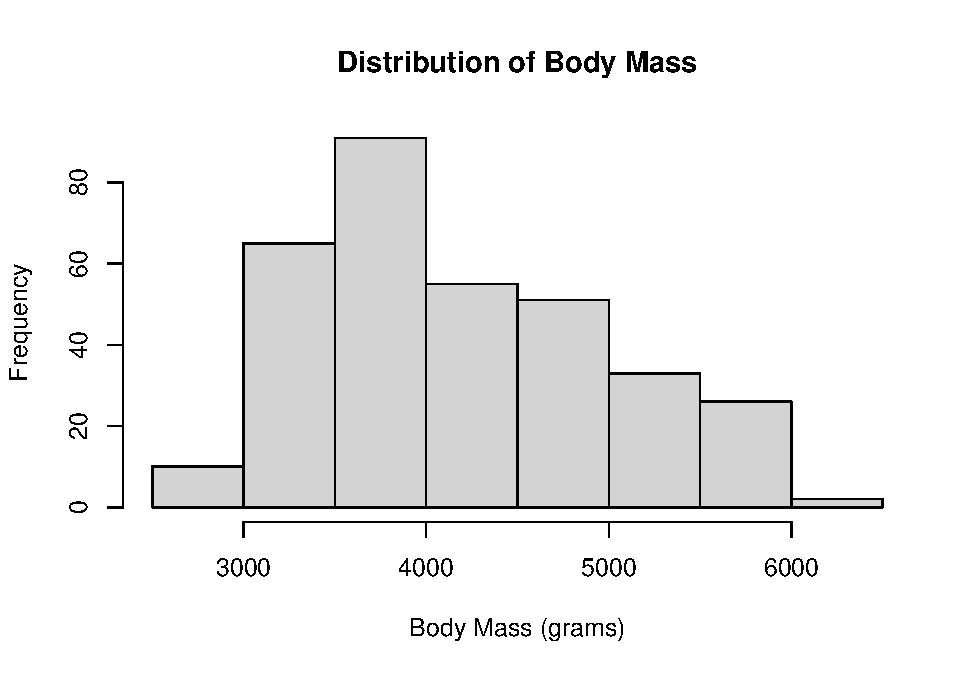
\includegraphics{Econ-Club-Example_files/figure-latex/base plotting-1.pdf}

The base plotting looks fine, but we can make more complex and
professional-looking figures using the \emph{ggplot2} package (included
in the tidyverse). ggplot2 can be a bit daunting at first, so we're
going to be using the \emph{ggpubr} package which is a wrapper for
ggplot2. We'll give up some customization options in exchange for a more
straight-forward experience. If you'd like to learn how to use the full
ggplot2 package (and I recommend you do), chapter 3 of \emph{R for Data
Science} is a great starting point.\\
\linebreak To make a histogram, we'll call the \texttt{gghistogram()}
function. This function asks us for our data and the variable seperately
so we don't have to use the \texttt{\$}. We'll add a bit of complexity
to this graph by setting \texttt{fill\ =\ "species"}. This will group
the data by species and create a histogram for each one. The resulting
figure will be all the histograms stacked on top of each other. This is
a good way to see how the distribution of body weight varies based on
species. Like before, the graph will appear in the \emph{plots} pane
where it can be exported.

\begin{Shaded}
\begin{Highlighting}[]
\FunctionTok{gghistogram}\NormalTok{(}\AttributeTok{data =}\NormalTok{ penguin, }\AttributeTok{x =} \StringTok{"body.mass.g"}\NormalTok{, }\AttributeTok{fill =} \StringTok{"species"}\NormalTok{,}
            \AttributeTok{title =} \StringTok{"Distribution of Body Mass"}\NormalTok{,}
            \AttributeTok{ylab =} \StringTok{"Frequency"}\NormalTok{,}
            \AttributeTok{xlab =} \StringTok{"Body Mass (grams)"}\NormalTok{)}
\end{Highlighting}
\end{Shaded}

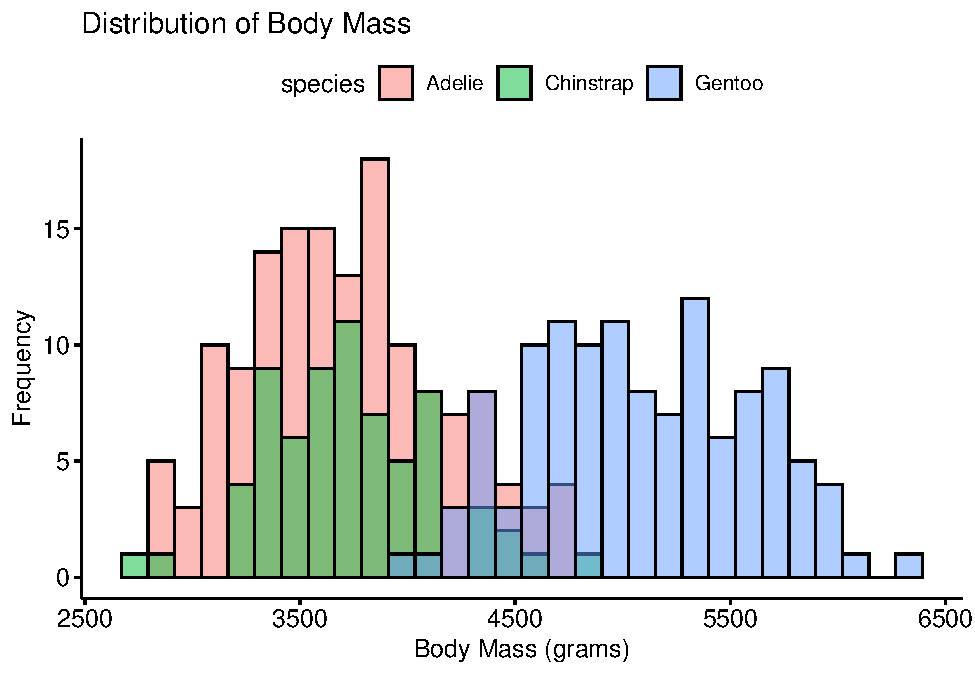
\includegraphics{Econ-Club-Example_files/figure-latex/ggpubr graph-1.pdf}

\hypertarget{regression}{%
\subsection{Regression}\label{regression}}

Fitting a regression model is also a common way to understand data. It
allows us to begin to quantify how variables interact and explain each
other. We'll fit a linear model using the \texttt{lm()} function. this
function first asks us for the formula of the model we want to fit in
the form \texttt{y\ \textasciitilde{}\ x1\ +\ x2\ +\ ...\ +xi}, then the
data where the variables are located. We assign this model to a variable
in the environment so we can use it later.

\begin{Shaded}
\begin{Highlighting}[]
\NormalTok{lm }\OtherTok{\textless{}{-}} \FunctionTok{lm}\NormalTok{(body.mass.g }\SpecialCharTok{\textasciitilde{}}\NormalTok{ flipper.length.mm }\SpecialCharTok{+}\NormalTok{ sex, }\AttributeTok{data =}\NormalTok{ penguin)}
\end{Highlighting}
\end{Shaded}

\pagebreak

The most rudimentary way to see the results of the regression is to use
the \texttt{summary()} function. This function will give you the usual
regression output, but it can be difficult to read and is not
publication ready.

\begin{Shaded}
\begin{Highlighting}[]
\FunctionTok{summary}\NormalTok{(lm)}
\end{Highlighting}
\end{Shaded}

\begin{verbatim}
## 
## Call:
## lm(formula = body.mass.g ~ flipper.length.mm + sex, data = penguin)
## 
## Residuals:
##     Min      1Q  Median      3Q     Max 
## -910.28 -243.89   -2.94  238.85 1067.73 
## 
## Coefficients:
##                    Estimate Std. Error t value Pr(>|t|)    
## (Intercept)       -5410.300    285.798 -18.931  < 2e-16 ***
## flipper.length.mm    46.982      1.441  32.598  < 2e-16 ***
## sexmale             347.850     40.342   8.623 2.78e-16 ***
## ---
## Signif. codes:  0 '***' 0.001 '**' 0.01 '*' 0.05 '.' 0.1 ' ' 1
## 
## Residual standard error: 355.9 on 330 degrees of freedom
## Multiple R-squared:  0.8058, Adjusted R-squared:  0.8047 
## F-statistic: 684.8 on 2 and 330 DF,  p-value: < 2.2e-16
\end{verbatim}

This is where a package like \emph{texreg} comes in. This package
contains a number of functions that will produce easier to read
regression output in a variety of formats.\\
To start, we have the \texttt{screenreg()} function. This just prints
the output to the console. It's not publication ready but is much easier
to read than \texttt{summary()}

\begin{Shaded}
\begin{Highlighting}[]
\FunctionTok{screenreg}\NormalTok{(lm)}
\end{Highlighting}
\end{Shaded}

\begin{verbatim}
## 
## ===============================
##                    Model 1     
## -------------------------------
## (Intercept)        -5410.30 ***
##                     (285.80)   
## flipper.length.mm     46.98 ***
##                       (1.44)   
## sexmale              347.85 ***
##                      (40.34)   
## -------------------------------
## R^2                    0.81    
## Adj. R^2               0.80    
## Num. obs.            333       
## ===============================
## *** p < 0.001; ** p < 0.01; * p < 0.05
\end{verbatim}

\pagebreak

To get a publication ready output, we can use the \texttt{texreg()} or
\texttt{htmlreg()} function. \texttt{texreg()} will generate the LaTeX
code for the table. \texttt{htmlreg()} will generate the html code for
the table. I'm using \texttt{texreg()} for this document since the
document is written in LaTeX.

\begin{Shaded}
\begin{Highlighting}[]
\FunctionTok{texreg}\NormalTok{(lm)}
\end{Highlighting}
\end{Shaded}

\begin{table}
\begin{center}
\begin{tabular}{l c}
\hline
 & Model 1 \\
\hline
(Intercept)       & $-5410.30^{***}$ \\
                  & $(285.80)$       \\
flipper.length.mm & $46.98^{***}$    \\
                  & $(1.44)$         \\
sexmale           & $347.85^{***}$   \\
                  & $(40.34)$        \\
\hline
R$^2$             & $0.81$           \\
Adj. R$^2$        & $0.80$           \\
Num. obs.         & $333$            \\
\hline
\multicolumn{2}{l}{\scriptsize{$^{***}p<0.001$; $^{**}p<0.01$; $^{*}p<0.05$}}
\end{tabular}
\caption{Statistical models}
\label{table:coefficients}
\end{center}
\end{table}

The far easier approach will be to use \texttt{htmlreg()} and save the
document as a .doc file that can be opened in Word.\\
The code would look something like
\texttt{htmlreg(model,\ file\ =\ "file/path/name.doc")}

\hypertarget{truthfulness-and-helpfulness}{%
\subsection{Truthfulness and
Helpfulness}\label{truthfulness-and-helpfulness}}

The final thing this document will cover is a reminder that you fully
explore the data before making conclusions.\\
Say we want to examine the relationship between the length and depth of
a penguin's bill. If we're not interested in the regression
coefficients, we can add the argument \texttt{add\ =\ "reg.line"} to
\texttt{ggscatter()} to fit the regression line
\texttt{y\ \textasciitilde{}\ x} to the scatter plot (if we wanted the
regression coefficients, we'd have to use the \texttt{lm()} function
discussed above).

\begin{Shaded}
\begin{Highlighting}[]
\FunctionTok{ggscatter}\NormalTok{(}\AttributeTok{data =}\NormalTok{ penguin, }\AttributeTok{x =} \StringTok{"bill.length.mm"}\NormalTok{, }\AttributeTok{y =} \StringTok{"bill.depth.mm"}\NormalTok{,}
          \AttributeTok{add =} \StringTok{"reg.line"}\NormalTok{,}
          \AttributeTok{title =} \StringTok{"Bill Length and Depth"}\NormalTok{)}
\end{Highlighting}
\end{Shaded}

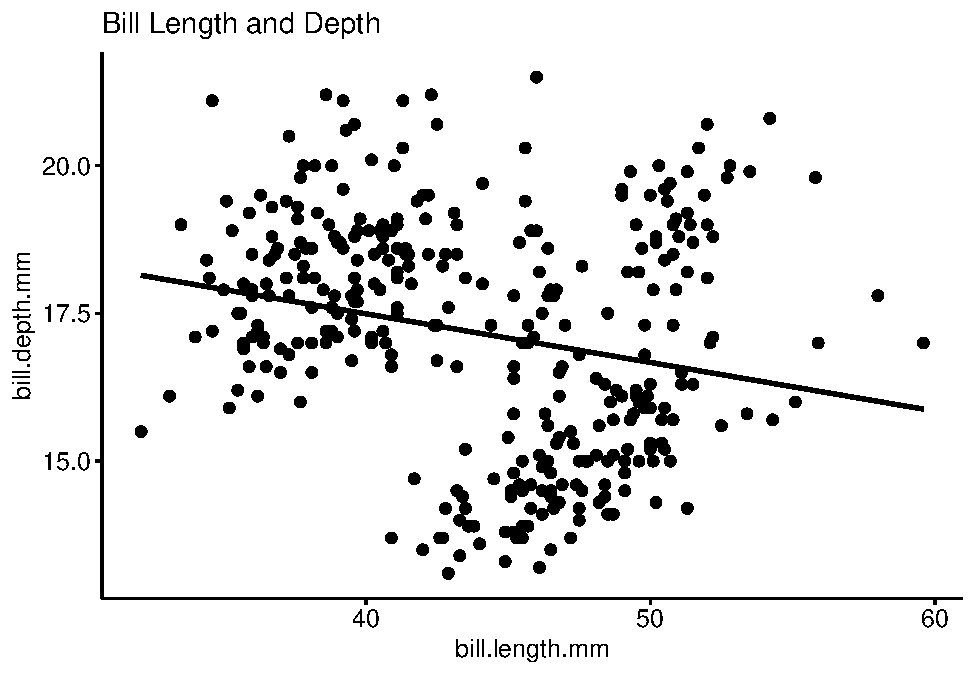
\includegraphics{Econ-Club-Example_files/figure-latex/Simpsons Paradox-1.pdf}

The regression shows a negative relationship between bill length and
depth. That's a bit odd. Especially if we look closer at the scatter
plot and see that the points appear to form a few distinct clumps. Is it
possible we missed something important? Let's break the data down by
species by adding the argument \texttt{color\ =\ "species"}. This will
color each point by its species and draw separate regression lines for
each species.

\begin{Shaded}
\begin{Highlighting}[]
\FunctionTok{ggscatter}\NormalTok{(}\AttributeTok{data =}\NormalTok{ penguin, }\AttributeTok{x =} \StringTok{"bill.length.mm"}\NormalTok{, }\AttributeTok{y =} \StringTok{"bill.depth.mm"}\NormalTok{, }\AttributeTok{color =} \StringTok{"species"}\NormalTok{,}
          \AttributeTok{add =} \StringTok{"reg.line"}\NormalTok{,}
          \AttributeTok{title =} \StringTok{"Bill Length and Depth by Species"}\NormalTok{)}
\end{Highlighting}
\end{Shaded}

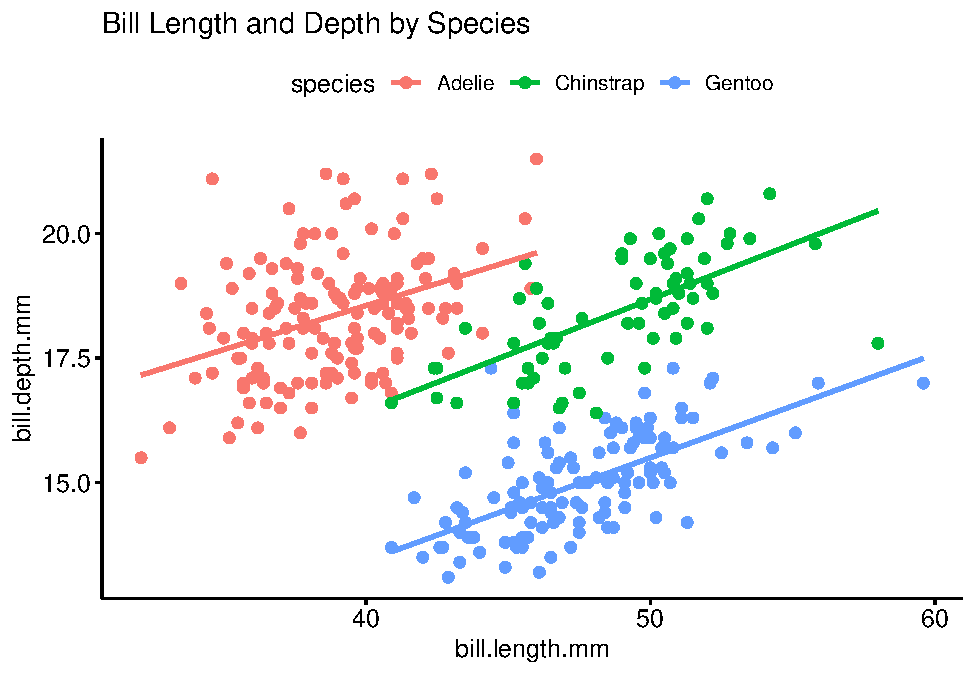
\includegraphics{Econ-Club-Example_files/figure-latex/Simpsons paradox 2-1.pdf}

Once we control for species, we see the relationship between bill length
and depth is actually positive! The clumping we saw earlier was penguin
species. If we look at the body mass histogram we made earlier, this
makes sense. the distribution of weight was quite different for each
species. If the penguins are different sizes, that could play a role in
their bill measurements.\\
This scenario where a trend will reverse when grouping is introduced is
known as \emph{Simpson's Paradox}. Not every dataset will behave like
this but it brings up an important conversation about truthfulness and
helpfulness.\\
Both graphs are factually correct but only one of them is helpful and
informative. When working with data, we need to be mindful that our
insights are both truthful and allows the audience to make an informed
decision.

\end{document}
